
\section{Introduction}
The \ac{TCA} implementation for the \ac{CMR} is one that heavily utilizes geometry and a rigid-body model assumption, while also placing an emphasis on relying on minimal assumptions/data about the environment and avoiding computationally complex calculations on input data from sensors, cameras, etc. There were various reasons as to why some of these assumptions/choices were made and why the agreed upon implementation was deemed the best choice for the given scenario. \cite{tractl} Figure~\ref{traction_control:algorithms:scarecrow} shows a testbed version of the \ac{CMR}.

\begin{figure}[htbp]
	\centering
	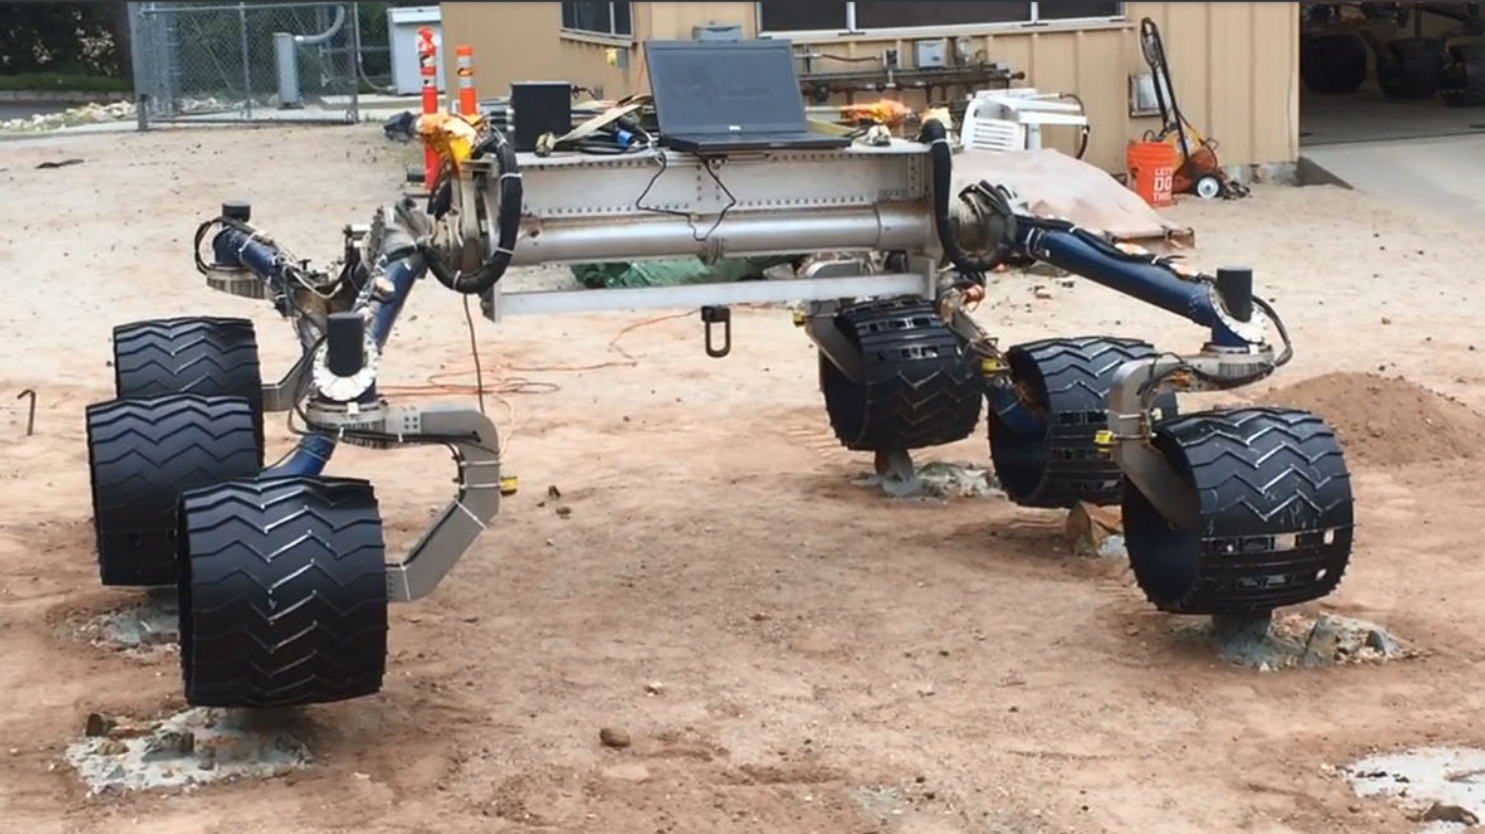
\includegraphics[width=.9\textwidth]{sections/algorithms/images/scarecrow_testbed.png}
	\caption{The Scarecrow Testbed Rover, a Rover Kinematically Similar to the \acl{CMR} \cite{tractl}}
	\label{traction_control:algorithms:scarecrow}
\end{figure}

\section{Design Limitations and Considerations}
It is important to note that the need for this \ac{TCA} was not discovered until after the flight system was actively engaging in its mission on the Martian surface, while ground control was observing telemetry of its use. Therefore, it was impossible to make any physical modifications to the \ac{CMR}, only software could be remotely flashed to it. \\

However, there are still ramifications to having this additional routine run on the \ac{CMR}. The limited computational resources available to do so must be considered carefully, so as to not interfere with existing processes being ran, and the implementation chosen has to have enough resources to perform the task it needs to as well. The team responsible for solving the problem at hand clarified some of these issues and how it restricted their choices for strategies to solve the problem. For example, the rover ``does not include force or torque sensors on the mobility subsystem, nor can it measure slip with high enough frequency to be able to react to it.'' \cite{tractl} \\

Some of the characteristics and assumptions of the \ac{CMR} and its \ac{TCA} implementation are discussed in the following sections.

\section{Ackermann Steering Model}\label{traction_control:algorithms:ackermann-steering-section}
Modeling vehicles using the Ackermann steering model is a common practice, including for the \ac{CMR}. Even thought it adds slightly more complex geometric modeling, the mechanical steering system can be implemented relatively easily, and there are benefits to doing so. \\

Figure~\ref{traction_control:algorithms:ackermann-steering} illustrates a basic vehicle that is modeled using Ackermann steering, where the left image has the wheels positioned such that the vehicle will move straight, while the right image would cause the vehicle to turn counter-clockwise. Important to note is that when in a turning position, the front wheels are not turned to the same angle as one another, because of the nonzero distance between them. They are positioned such that the direction that both wheels are pointing are normal to a common center point called the \ac{ICC}, so that when the vehicle turns, the left and right wheels follow two different circular arcs, but both of their centers are at the \ac{ICC}.

\begin{figure}[H]
	\centering
	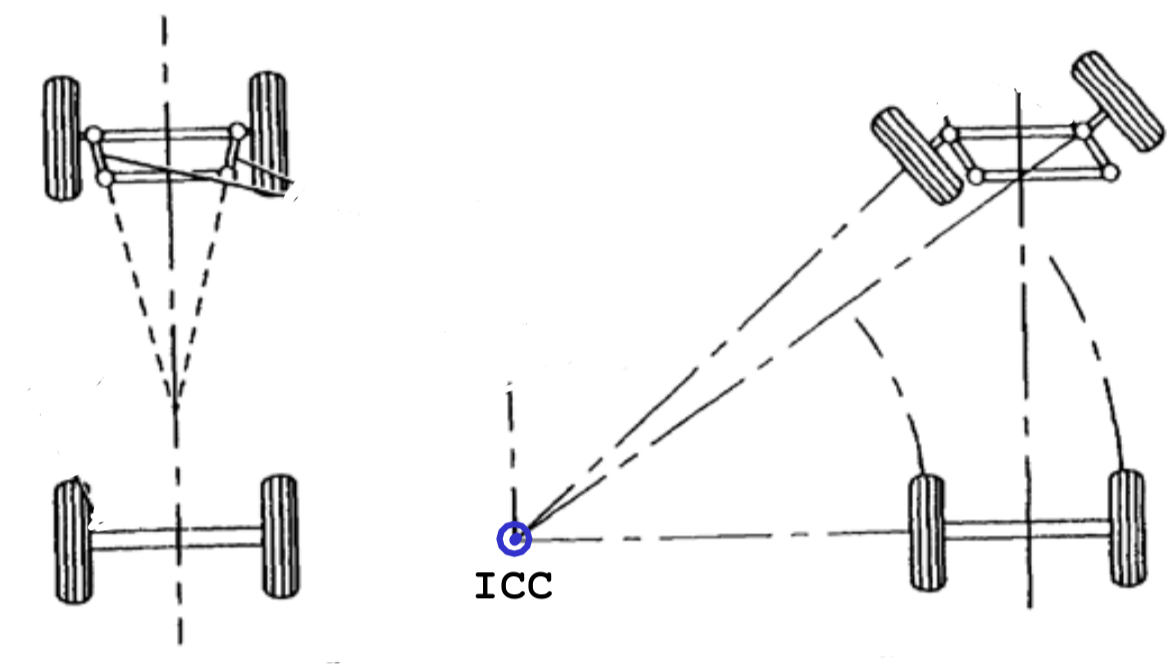
\includegraphics[width=.9\textwidth]{sections/algorithms/images/ackermann_steering.png}
	\caption{A Vehicle with Ackermann Steering Going Straight (Left) and in a Turning Position(Right)}
	\label{traction_control:algorithms:ackermann-steering}
\end{figure}

The benefit to this is that, assuming all the wheels' velocities are coordinated and in an ideal world, at no point while traveling in these flat, circular arcs will a wheel slip. Less slippage means less unpredictable behavior, such as a wheel slipping over a rough surface. However, the assumption that the \ac{CMR} would only be traversing terrain that could be modeled as flat is what led to the need for the \ac{TCA}, as excessive slippage occurred due to the reality that the terrain was non-negligible. As one wheel would traverse over a rock and then back down, it traveled a longer distance. \\

The Ackermann steering model by itself does not account for this extra distance and this caused the wheel slippage, which damaged them at an alarming rate. This is how the \ac{TCA} can be used to improve the model, so that when rough terrain is being traversed, the wheel(s) doing so can be sped up accordingly.

\section{Rigid-Body Model Assumption}\label{traction_control:algorithms:rigid-body}
The rigid-body model assumption says that a body of some sturdy material can be assumed to maintain it shape, and that a force/torque that it can expect to encounter will not deform it to a degree that needs to be accounted for. This is not true in reality, but in scenarios like these, the deformation can be negligible. \\

Making this assumption can be extremely beneficial when implementing an algorithm like \ac{TCA} because it heavily simplifies the math needed to represent vectors in different coordinate frames.

\section{Coordinate Frame Notation}
%
%TO-DO, add: \\
% 1.) description of what a coordinate frame is and why they're used \\
% 2.) \ac{CMR} frame notation \\
% 3.) mention differences in \ac{SRR} frames \\
% 4.) maybe more \\

Coordinate frames are useful in robotics for the purpose of keeping track of the robot positions, orientations, and velocities in space. These frames can be translated from  a reference to another frame, such as from the base robot frame to each individual leg frame. Robotics often uses Cartesian coordinates, so the coordinate frames are created with an origin, x, y, and z axes. \\

To be able to show the relative position and orientation of one frame to another, geometric relationships between them need to be found. A rotation matrix can be used to show the relative orientation between two frames. For example, the orientation of the 1st frame $o_{1}x_{1}y_{1}z_{1}$ with respect to the base frame $o_{0}x_{0}y_{0}z_{0}$ can be written with the rotation matrix:
\begin{equation}\label{traction_control:algorithms:r01}
	R^{0}_{1} = [x^{0}_{1} | y^{0}_{1} | z^{0}_{1}]
\end{equation}

One way to compute the rotation matrix is with the entries being in terms of angle $\theta$. The second way is to project the 1st frame on the 0 frame which uses the dot product.  The dot products with respect of the 1st frame onto the 0 frame can be shown as
\begin{equation}
	x^{0}_{1} = \left[\begin{array}{c}
				x_{1}\cdot x_{0} \\
			    x_{1}\cdot y_{0} \\
			    x_{1}\cdot z_{0}
				\end{array} \right],
			%
	y^{0}_{1} = \left[\begin{array}{c}
				y_{1}\cdot x_{0} \\
				y_{1}\cdot y_{0} \\
				y_{1}\cdot z_{0}
	\end{array} \right],
			%
	z^{0}_{1} = \left[\begin{array}{c}
				z_{1}\cdot x_{0} \\
				z_{1}\cdot y_{0} \\
				z_{1}\cdot z_{0}
	\end{array} \right]
\end{equation}

There are three basic rotation matrices- about the x-axis, y-axis, and z-axis. With respect to angle $\theta$, these rotation matrices are defined in
Equations~\ref{traction_control:algorithms:rx}, \ref{traction_control:algorithms:ry}, \ref{traction_control:algorithms:rz}. 
These 3 rotations are also called the roll$(\phi)$, pitch $(\theta)$, and yaw$(\psi)$ matrices. The order of rotation is through yaw (x,$(\psi)$),pitch (y,$(\theta)$), and roll (z,$(\phi)$. \\

\begin{equation}
	R_{x,\theta} = \left[\begin{array}{ccc}
				1 & 0 & 0 \\
				0 & cos(\theta) & -sin(\theta)  \\
				0 & sin(\theta) & cos(\theta) 
				\end{array}\right]
	\label{traction_control:algorithms:rx}
\end{equation}

\begin{equation}
	R_{y,\theta} = \left[\begin{array}{ccc}
		cos(\theta) & 0 & sin(\theta) \\
		0 & 1 & 0 \\
		-sin(\theta) & 0 & cos(\theta) 
	\end{array}\right]
	\label{traction_control:algorithms:ry}
\end{equation}

\begin{equation}
	R_{z,\theta} = \left[\begin{array}{ccc}
		cos(\theta) & sin(\theta) & 0 \\
		sin(\theta) & cos(\theta) & 0 \\
		0 & 0 & 1 \\
	 
	\end{array}\right]
	\label{traction_control:algorithms:rz}
\end{equation}\\

After finding both the position and orientation of a frame, they can be put into a homogeneous transformation matrix. This can comprise of a series of rigid motions, which are pure translations and pure rotations only. The transformation matrix consists of the rotation between the frames (top 3x3), the distance (right 3x1 column vector), and the bottom row being matrix identity to allow a series of multiplications. Figure~\ref{traction_control:algorithms:basicT} shows the homogeneous transformation matrix. 

\begin{equation}
	H^{0}_{n} = \left[\begin{array}{cc}
			R^{0}_{n} & d^{0}_{n}\\
			0 & 1 
			\end{array}\right]
		\label{traction_control:algorithms:basicT}
\end{equation}


The rover, like any robot, has coordinate frames to define its position and rotation matrices.
 Figure~\ref{traction_control:algorithms:coordinates-side} shows these frames from the left side of the robot. A top view is also provided as Figure~\ref{traction_control:algorithms:coordinates-top}.

\begin{figure}[H]
	\centering
	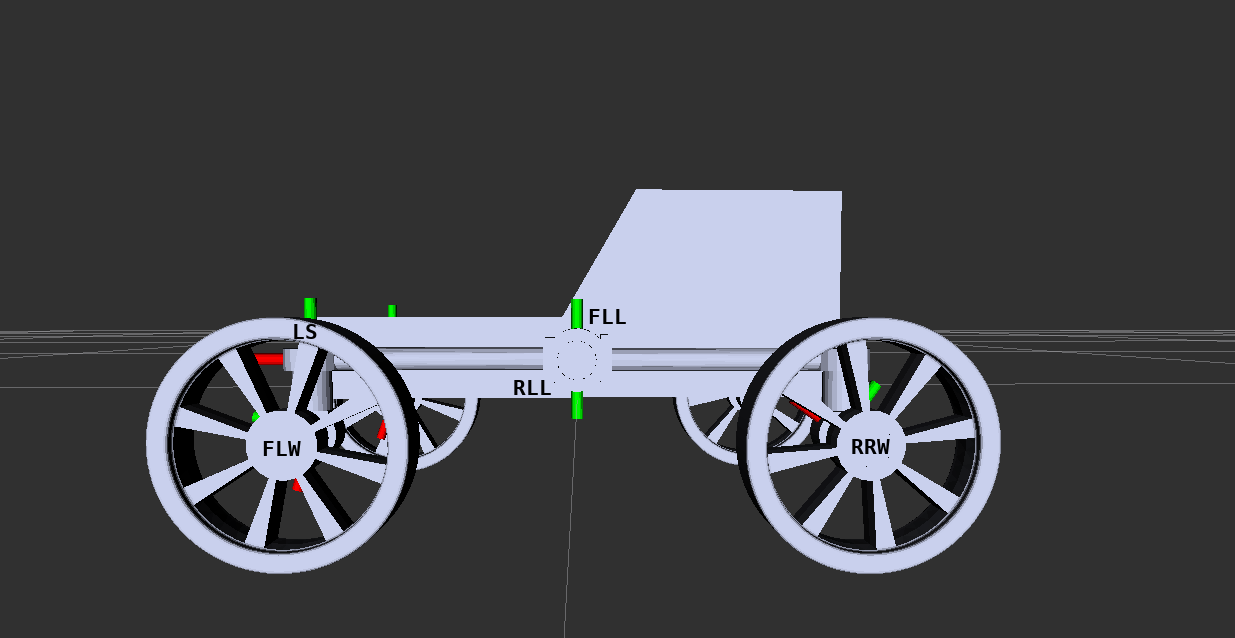
\includegraphics[scale=0.35, width=.7\textwidth]{sections/algorithms/images/srr_side.png}
	\caption{Side View of the Robot Model and its Coordinate Frames}
	\label{traction_control:algorithms:coordinates-side}
\end{figure}
 
\begin{figure}[H]
	\centering
	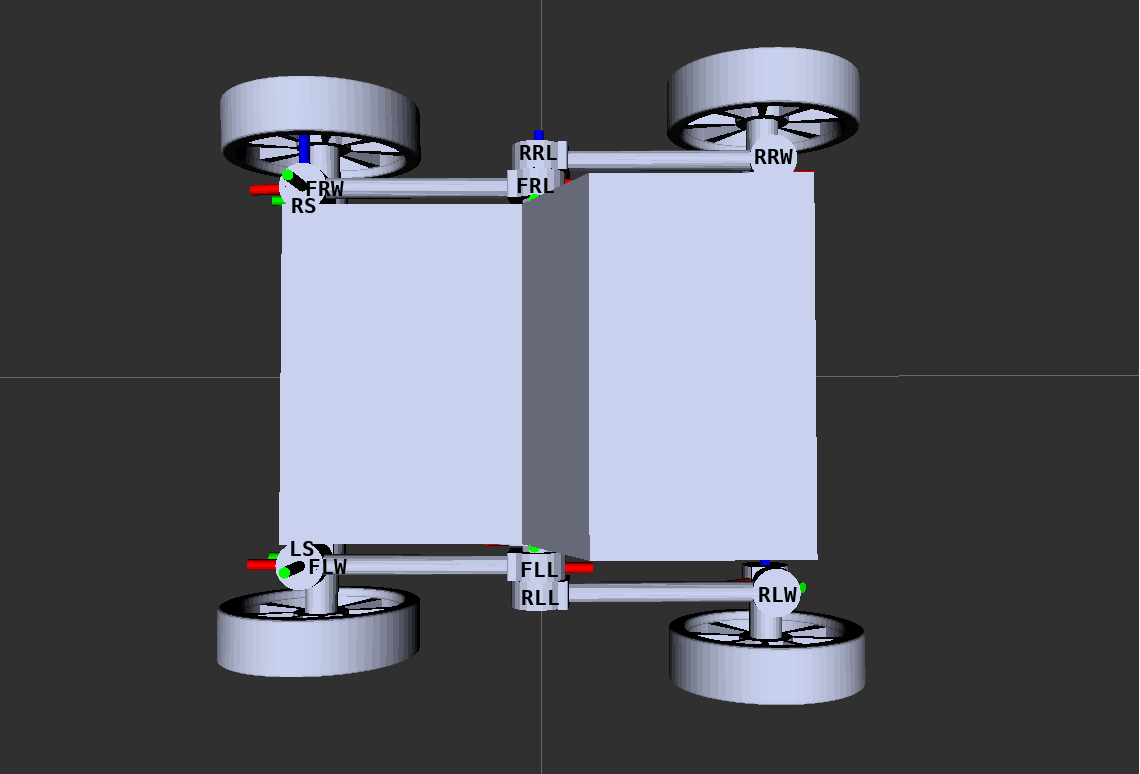
\includegraphics[scale=0.3]{sections/algorithms/images/srr_top.png}
	\caption{Side View of the Robot Model and its Coordinate Frames}
	\label{traction_control:algorithms:coordinates-top}
\end{figure}
 
A summary of the acronyms for the coordinate frames used in Figures~\ref{traction_control:algorithms:coordinates-side} and~\ref{traction_control:algorithms:coordinates-top} are seen below in Table~\ref{table:1}.
\begin{table}[H]
\begin{center}
	\begin{tabular}{|c|c|} 
		\hline    
		Label & Name \\
		\hline
		FLL & Front Left Leg \\
		FRL & Front Right Leg \\
		RLL & Rear Left Leg \\
		RRL & Rear Right Leg \\
		FLW & Front Left Wheel \\
		FRW & Front Right Wheel \\
		RLW & Rear Left Wheel \\
		RRW & Rear Right Wheel \\
		LS  & Left Steering \\ 
		RS  & Right Steering \\ 
	    \hline
	\end{tabular}
 	\caption{\label{table:1} Table of Acronyms for Model Axes}  	
\end{center}
\end{table}

The rover model can be drawn to show its geometry in a simple manner. Depicted from its side, there is the pivot joint from the chassis in the center. Two legs are connected to the the center pivot joint. The front leg also has a revolute joint at its end to be able to steer the front wheels.

The difference between this model and the Curiosity Rover is that the Curiosity Rover has a third leg, which can be defined as the rocker joint and bogie joints. The legs are designed much differently as compared to the early model of the Sample-Return Rover. The SRR only has the center pivot joint.

As seen in Figure~\ref{traction_control:algorithms:side-diagram},the diagram is of the left side of the rover, and the front is facing left. Wheel centers are denoted with $A_{i}$. The lengths of each leg are shown with $l_{i}$. Angles of specific areas are denoted by either $\psi$, k, or $\delta$. 


\begin{figure}[H]
	\centering
	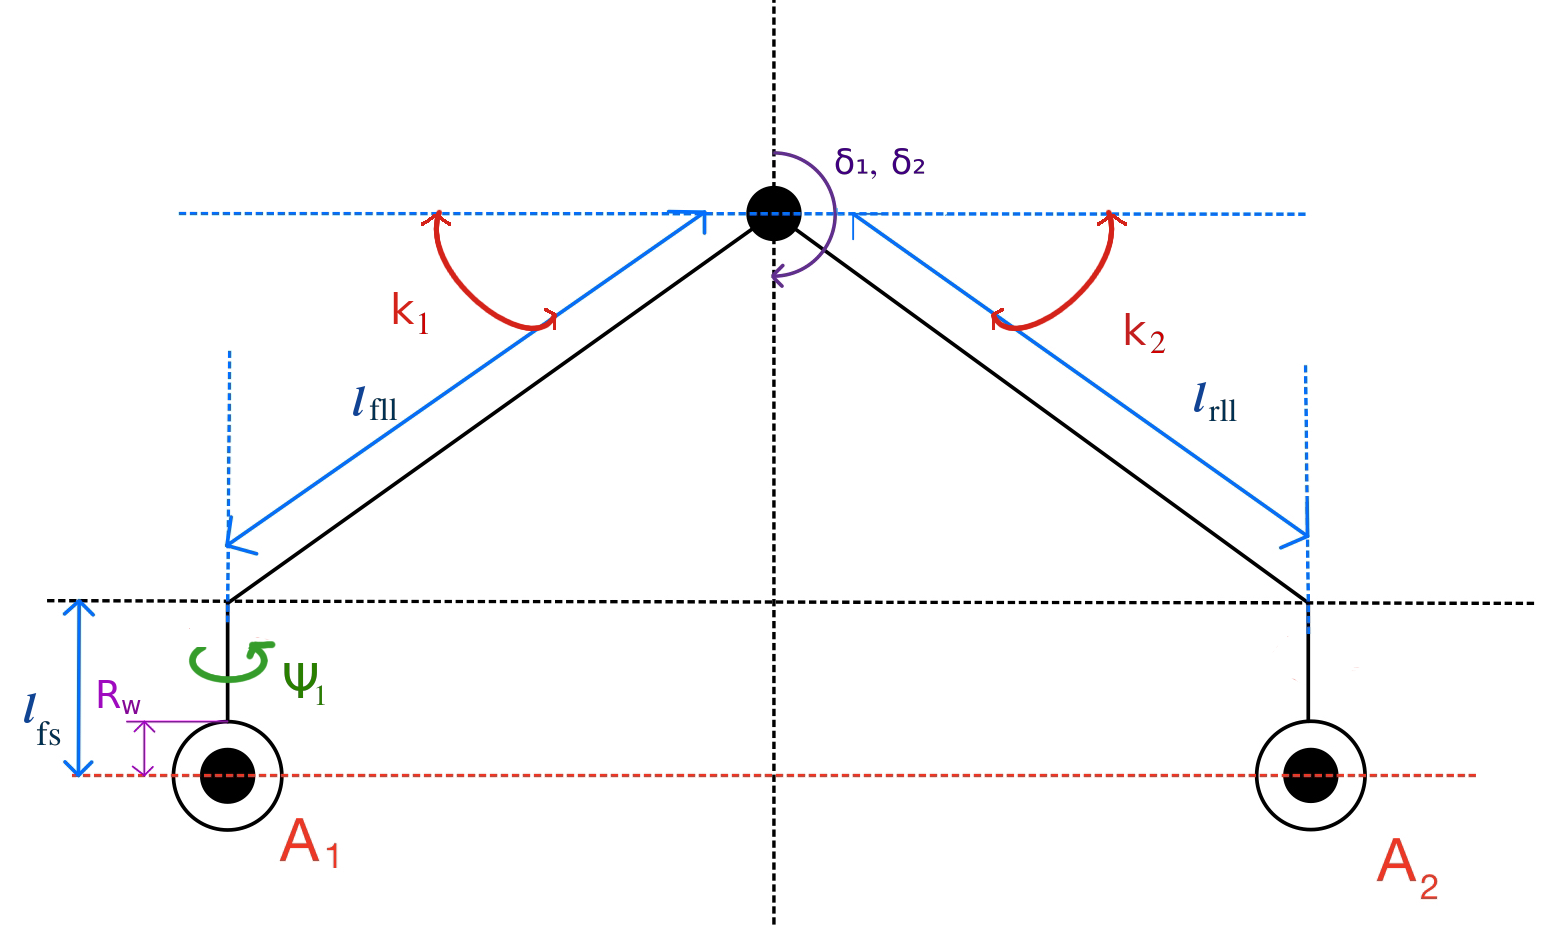
\includegraphics[scale=0.3]{sections/algorithms/images/side-diagram.png}	
	\caption{Side Diagram of the Rover Model on Flat Ground}	
	\label{traction_control:algorithms:side-diagram}
\end{figure}

\begin{table}[H]
\begin{center}\label{table:2}
	\begin{tabular}{| >{\centering\arraybackslash} m{1.2in} | >{\centering\arraybackslash} m{4.5in} |} 
		\hline
		Symbol & Description \\
		\hline
		A1 & Wheel 1 - Front Left \\
		A2 & Wheel 2 - Rear Left \\
		$R_{w}$ & Wheel Radius \\
		$\psi_{1}$ & Front Steering Angle \\
		$k_{1}$ & Angle between Front Leg and Chassis x-axis on Flat Ground \\
		$k_{2}$ & Angle between Rear Leg and Chassis x-axis on Flat Ground \\
		$l_{fs}$ & Front Steering Leg Length \\ 
		$l_{fll}$ & Front Left Leg Length \\ 
		$l_{rll}$ & Rear Left Leg Length \\ 
		$\delta_{1}$ & Front Left Leg Pivot Angle    \\
		$\delta_{2}$ & Rear Left Leg Pivot Angle   \\
		\hline
	
	\end{tabular}
\caption{Description of Symbol Nomenclature}
\end{center}
\end{table}


\section{Algorithms}
\subsection{Overview}
The following subsections explains the \ac{TCA} in more detail, including its data flow, how this data is acquired, and the derivations for concepts integral to its implementation.

\subsection{Inputs and Outputs}
The \ac{TCA} operates on a number of configuration parameters, values which do not change over time. Most of these have to do with the size and shape of the vehicle (i.e., the lengths of links between joints), which obviously is staticas time passes. The algorithm also relies on inputs that are to be updated every time step (each time the algorithm calculates its outputs), which are summarized in Tables~\ref{traction_control:algorithms:inputs-cmr} and~\ref{traction_control:algorithms:inputs-srr} for an implementation onboard the \ac{CMR} and \ac{SRR}, respectively.

\begin{table}[H]
	\centering
	\begin{tabular}{| >{\centering\arraybackslash} m{1.2in} | >{\centering\arraybackslash} m{4.5in} |}
		\hline
		\textbf{Input Value} & \textbf{Description} \\
		\hline
		$\vec{\omega}$ & The 3x1 angular velocity vector around the base coordinate frame of the vehicle \\
		\hline
		$\vec{\delta}=\left[\beta, \rho_{1}, \rho_{2}\right]^{T}$ & The 3x1 vector of joint positions describing the rotation of the bogie joint and each rocker joint \\
		\hline
		$\vec{\dot{\delta}}=\left[\dot{\beta}, \dot{\rho_{1}}, \dot{\rho_{2}}\right]^{T}$ & The 3x1 vector of joint velocities describing the rotational speed of the bogie joint and each rocker joint \\
		\hline
		$\vec{\Psi}$ & The 6x1 vector of joint positions describing the steering angle of each wheel \\
		\hline
	\end{tabular}
	\caption{Summary of the Inputs for the Algorithm Onboard the Curiosity Mars Rover}
	\label{traction_control:algorithms:inputs-cmr}
\end{table}

\begin{table}[H]
	\centering
	\begin{tabular}{| >{\centering\arraybackslash} m{1.2in} | >{\centering\arraybackslash} m{4.5in} |}
		\hline
		\textbf{Input Value} & \textbf{Description} \\
		\hline
		$\vec{\dot{\theta}}$ & The 6x1 vector of joint speeds to be commanded to each of the vehicle's wheels \\
		\hline
	\end{tabular}
	\caption{Summary of the Inputs for the Algorithm Onboard the Curiosity Mars Rover}
	\label{traction_control:algorithms:outputs-cmr}
\end{table}

When considering the algorithm for the \ac{SRR}, the inputs and outputs will only change because the number of suspension joints and wheels differs from the \ac{CMR}. Otherwise, the idea is the same. The inputs and outputs for an \ac{SRR} implementation are summarized in Tables~\ref{traction_control:algorithms:inputs-srr} and~\ref{traction_control:algorithms:outputs-srr}.

\begin{table}[H]
	\centering
	\begin{tabular}{| >{\centering\arraybackslash} m{1.2in} | >{\centering\arraybackslash} m{4.5in} |}
		\hline
		\textbf{Input Value} & \textbf{Description} \\
		\hline
		$\vec{\omega}$ & The 3x1 angular velocity vector around the base coordinate frame of the vehicle \\
		\hline
		$\vec{\delta}$ & The 4x1 vector of joint positions describing the rotation of the joints corresponding to each of the four legs' pivot points \\
		\hline
		$\vec{\dot{\delta}}$ & The 4x1 vector of joint velocities describing the rotational speed of the joints corresponding to each of the four legs' pivot points \\
		\hline
		$\vec{\Psi}$ & The 4x1 vector of joint positions describing the steering angle of each wheel \\
		\hline
	\end{tabular}
	\caption{Summary of the Inputs for the Algorithm Onboard the Curiosity Mars Rover}
	\label{traction_control:algorithms:inputs-srr}
\end{table}

\begin{table}[H]
	\centering
	\begin{tabular}{| >{\centering\arraybackslash} m{1.2in} | >{\centering\arraybackslash} m{4.5in} |}
		\hline
		\textbf{Input Value} & \textbf{Description} \\
		\hline
		$\vec{\dot{\theta}}$ & The 6x1 vector of joint speeds to be commanded to each of the vehicle's wheels \\
		\hline
	\end{tabular}
	\caption{Summary of the Inputs for the Algorithm Onboard the Curiosity Mars Rover}
	\label{traction_control:algorithms:outputs-srr}
\end{table}

\subsection{Measuring the Inputs}

As seen in Tables~\ref{traction_control:algorithms:inputs-cmr} and~\ref{traction_control:algorithms:inputs-srr}, the \ac{TCA} has four inputs, each of which are measured/calculated each time step. The \ac{CMR} was equipped with encoders on each joint, so because the inputs $\vec{\delta}$ and $\vec{\Psi}$ are joint position measurements, their values are gathered directly from each of the respective encoders. Absolute encoders are able to output a position relative to some coordinated "home/zero" position, which is what are utilized here. \\

Some encoders are also capable of measuring the instantaneous velocity of their respective joint, but the team behind this solution for the \ac{TCA} did not have these available on the \ac{CMR} to collect the values of $\vec{\dot{\delta}}$. It was clarified that the velocities of these joints were calculated as a time derivative \cite{tractl}. This means that given the initial and final position $\alpha$ of a joint which rotated over a small length of time $\Delta t$, the velocity of the joint at its final position can be estimated as follows:

\begin{equation}
	\dot{\alpha} \approx \dot{\alpha}_{avg} = \frac{\alpha_{f} - \alpha_{i}}{\Delta t}
\end{equation}

The angular velocity vector $\vec{\omega}$ of the \ac{CMR} was calculated using an \ac{IMU}, and more specifically the digital readings off the gyroscope(s) inside of it. A gyroscope, a 3D rendering of which can be seen in Figure~\ref{traction_control:algorithms:gyro}, is a three degree of freedom mechanism which allows for the measurement of independent rotation about the three principal axes. With an \ac{IMU} mounted to the body of the vehicle, $\vec{\omega}$ is easily measured.

\begin{figure}[htbp]
	\centering
	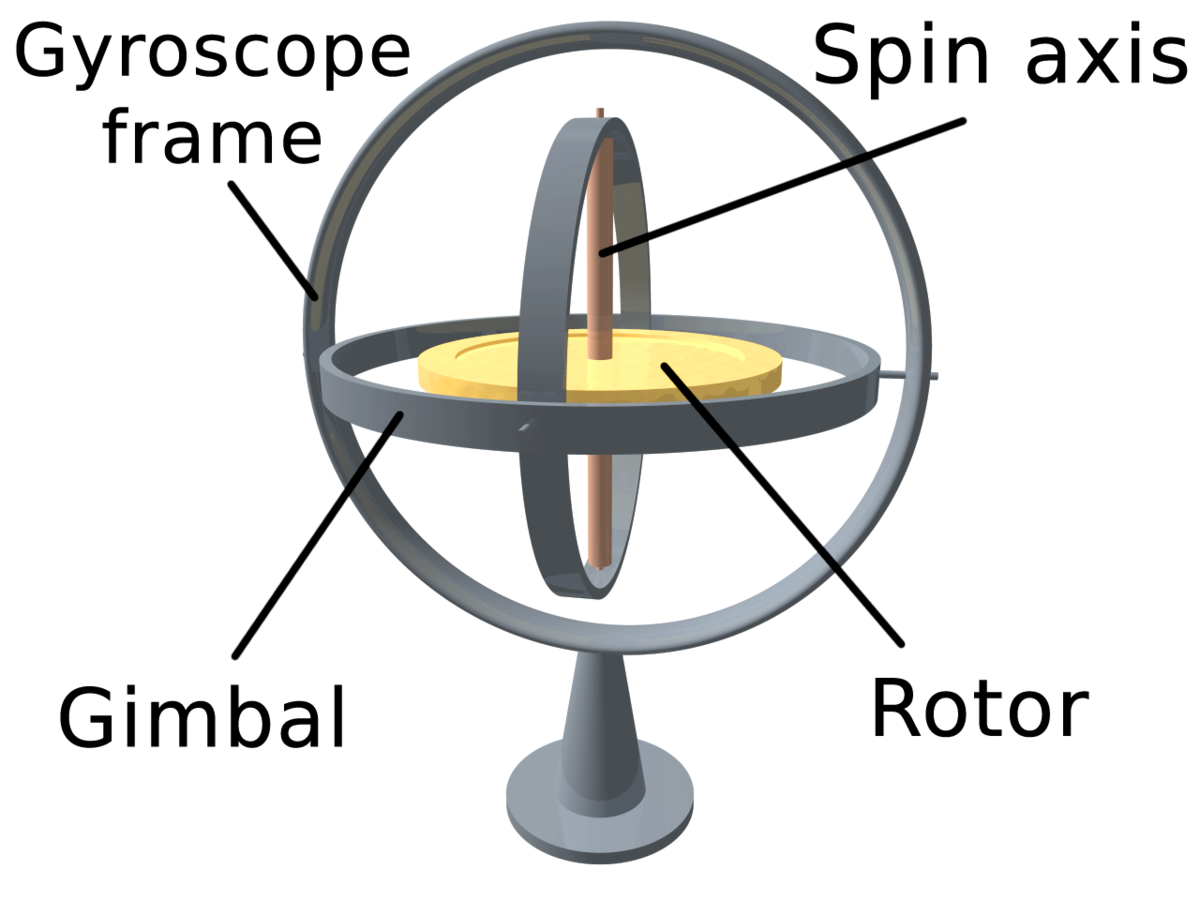
\includegraphics[width=.5\textwidth]{sections/algorithms/images/gyroscope.png}
	\caption{A 3D Rendering of a Gyroscope}
	\label{traction_control:algorithms:gyro}
\end{figure}

\subsection{Transferring Velocity Between Coordinate Frames}\label{traction_control:algorithms:transferring-velocity}
This implementation for \ac{TCA} is a largely geometric solution in the sense that a majority of the calculations it performs is estimating the linear velocity of each wheel given the knowledge of the vehicle's overall linear and angular velocity and the velocity of the joints intermediate to the vehicle's body and that wheel. Therefore, it is important to understand how these types of vectors interact with one another. \\

Consider some coordinate frames G and H which are attached to separate rigid-bodies as described in Section~\ref{traction_control:algorithms:rigid-body}. Now consider some point Q that is resolved in frame H. The motion of Q is trivial to resolve in H, but what if the motion of Q needs to be resolved in G? First consider the case where the frames G and H are coincident and the position of their origins do not change with time, but there is a nonzero rotational velocity of H relative to G called ${}^{G}_{H}\Omega$. Assuming the point Q has no velocity relative to H, the linear velocity induced by this rotation resolved in G can be calculated as follows \cite{craig}:

\begin{equation}
	{}^{G}V_{Q} = {}^{G}_{H}\vec{\omega} \times \left({}^{G}_{H}R \cdot {}^{H}Q\right) \text{, when } {}^{H}V_{Q} = 0_{3x1}
\end{equation}

In other words, the linear velocity of Q resolved in G is equal to the cross product of the rotational velocity of H relative to G and the position of Q resolved in G. Now, consider that there is a nonzero linear velocity of Q relative to H. This is simply rotated into the frame G, so the expression expands to the following \cite{craig}:

\begin{equation}\label{traction_control:algorithms:VQG}
	{}^{G}V_{Q} = \left({}^{G}_{H}R \cdot {}^{H}V_{Q}\right) + \left({}^{G}_{H}\vec{\omega} \times \left({}^{G}_{H}R \cdot {}^{H}Q\right)\right)
\end{equation}

In the general case, there are more considerations to take to fully formulate how linear velocities are transferred across frames \cite{craig}. However, none of them need be considered for this scenario because they are unique to the fact that G and H are assumed to be attached to separate rigid bodies. In the context of this algorithm, all frames are known to be attached to the same rigid body (the rover). Therefore, when solving for the velocity of a frame relative to another, both attached to the rover, Equation~\ref{traction_control:algorithms:VQG} will fully define that solution.

\subsection{Contact Angle Frame}\label{traction_control:algorithms:contact-angle-section}
As mentioned in Section~\ref{traction_control:algorithms:ackermann-steering-section}, basic Ackermann Steering is typically used to model a vehicle assumed to be traversing a planar surface, or at least a terrain whose inconsistencies are negligible. The \ac{TCA} acknowledges that is not the case here by defining this contact angle frame relative to each wheel's frame, an illustration of which can be seen in Figure~\ref{traction_control:algorithms:contact-angle}.

\begin{figure}[H]
	\centering
	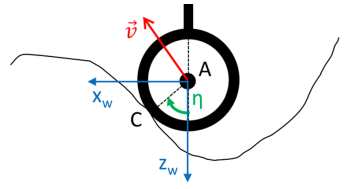
\includegraphics[width=.8\textwidth]{sections/algorithms/images/contact_angle.png}
	\caption{The Contact Angle $\eta$ Defines the Contact Wheel Frame for Some Wheel A \cite{tractl}}
	\label{traction_control:algorithms:contact-angle}
\end{figure}

XXXXXXXXXXXXXXXXXX
ADD FIGURE REF HERE
XXXXXXXXXXXXXXXXXX \\
Figure~\ref{traction_control:algorithms:contact-angle} uses the vector $\vec{v}$ to denote the linear velocity of the wheel A, which is calculated using the concept of velocity transformation introduced in Section~\ref{traction_control:algorithms:transferring-velocity}. The geometry of the \ac{CMR} is symmetrical across the body's x-axis (front to back), but asymmetrical across its width (side to side), as can be seen in Figure~\ref{}. This implies that while the theory of velocity transformation applies to both, the specific calculations to accomplish this for one wheel is slightly different than some others. For example, the calculation of a wheel linked to the rocker joint can be seen in Equation~\ref{traction_control:algorithms:velocity-rocker-wheel}, while the calculation for one of the wheels linked to one of the bogie pivot joints can be seen in Equation~\ref{traction_control:algorithms:velocity-bogie-wheel} \cite{tractl}. Essentially, the velocity is transferred an additional time because there is another joint intermediate to the bogie wheels that cannot be ignored. \\

\begin{equation}\label{traction_control:algorithms:velocity-body}
	{}^{bd}V_{D} = \left[\begin{array}{c}
		\dot{x}_0 \\
		0 \\
		0
	\end{array}\right] + \left(\left[\begin{array}{c}
		\omega_{x} \\
		\omega_{y} \\
		\omega_{z}
	\end{array}\right] \times \left[\begin{array}{c}
	x_{od} \\
	0 \\
	z_{od}
	\end{array}\right]\right)
\end{equation}

\begin{equation}\label{traction_control:algorithms:velocity-rocker-wheel}
	{}^{bd}V_{A_{1}} = {}^{bd}V_{D} - \left[\begin{array}{c}
		\omega_{x} \\
		\omega_{y} + \dot{\beta} \\
		\omega_{z}
	\end{array}\right] \times \left({}^{bd}_{rk1}R \cdot \left[\begin{array}{c}
		-l_{fd} cos(\kappa_{1}) \\
		-Y_{of} \\
		-l_{fd} sin(\kappa_{1})
	\end{array}\right]\right)
\end{equation}

\begin{equation}\label{traction_control:algorithms:velocity-bogie}
	{}^{bd}V_{B_{1}} = {}^{bd}V_{D} - \left[\begin{array}{c}
		\omega_{x} \\
		\omega_{y} + \dot{\beta} \\
		\omega_{z}
	\end{array}\right] \times \left({}^{bd}_{rk1}R \cdot \left[\begin{array}{c}
		l_{db} cos(\kappa_{2}) \\
		0 \\
		-l_{fd} sin(\kappa_{2})
	\end{array}\right]\right)
\end{equation}

\begin{equation}\label{traction_control:algorithms:velocity-bogie-wheel}
	{}^{bd}V_{A_{3}} = {}^{bd}V_{B_{1}} - \left[\begin{array}{c}
		\omega_{x} \\
		\omega_{y} + \dot{\beta} + \dot{\rho}_{1} \\
		\omega_{z}
	\end{array}\right] \times \left({}^{bd}_{rk1}R \cdot {}^{rk1}_{bg1}R \cdot \left[\begin{array}{c}
		-l_{bm} cos(\kappa_{3}) \\
		Y_{om} \\
		-l_{bm} sin(\kappa_{3})
	\end{array}\right]\right)
\end{equation}

See \cite{tractl} for a more detailed explanation as to the meaning of each variable in Equations~\ref{traction_control:algorithms:velocity-body}-\ref{traction_control:algorithms:velocity-bogie-wheel}. With an understanding of those variables, it can be seen that these variables follow the general form of Equation~\ref{traction_control:algorithms:VQG}. \\

For those calculations to be performed, the linear velocity of the rover's body must be estimated. One of the existing requirements for the \ac{CMR} is that at least one of its wheels must be operating at its peak speed at all times (other than when it is stationary). This requirement along with the assumption that the rover is moving in the rover body's x-axis (forward or backward) means that its linear velocity can be assumed to be completely in its x-axis. This is where the initial linear velocity value $\left[\dot{x}_0 \;\; 0 \;\; 0\right]^{T}$ comes from in Equation~\ref{traction_control:algorithms:velocity-body}. \\

Once the linear velocities of the six wheels resolved to the rover's body frame, ${}^{bd}V_{A_{1-6}}$, are calculated, the contact angle $\eta_{i}$ can be solved for the $i^{th}$ wheel. The $i^{th}$ contact angle frame is defined as coincident with the $i^{th}$ wheel frame (their origins are the same) with a rotation of $\eta_{i}$ about the same axis that wheel rotates about, $Y_{w_{i}}$. It can be seen in Figure~\ref{traction_control:algorithms:contact-angle} that the linear velocity of the wheel is perpendicular to this contact angle frame, so the calculation for finding $\eta_{i}$ is straightforward:

\begin{equation}\label{traction_control:algorithms:contact-angle-i}
	\eta_{i} = -\arctan\left(\frac{{}^{w_{i}}V^{z}_{A_{i}}}{{}^{w_{i}}V^{x}_{A_{i}}}\right)
\end{equation}

\subsection{Solving for Commanded Wheel Rates}\label{traction_control:algorithms:solving-wheel-rates}
In the general case, the objective is to find the wheel rates given some desired velocity of the rover. When calculating the contact angle frames for each wheel, it was proven that the linear velocity of the rover can be resolved in the wheel frames, while accounting for velocities induced by angular velocities from joint motions. That calculation was performed for the current estimated linear velocity of the vehicle, but now the same routine can be done to calculate the linear velocities of the wheels that would achieve this objective linear velocity of the rover body. In other words, Equations~\ref{traction_control:algorithms:velocity-body}-\ref{traction_control:algorithms:velocity-bogie-wheel} (and those required for the other wheels, left out in the interest of brevity) can be reused other than the fact that the initial velocity in Equation~\ref{traction_control:algorithms:velocity-body} will no longer be $\left[\dot{x}_0 \;\; 0 \;\; 0\right]^{T}$ but this objective velocity. \\

By itself, calculating this linear velocity of the wheels is not beneficial, but it can be built onto to calculate the angular velocity of the wheel required to generate its desired linear velocity, thereby solving the problem. To do this, the linear velocity of the wheel with respect to the rover's body frame must be transformed to the linear velocity of the contact angle frame, as seen in Equation~\ref{traction_control:algorithms:trans-vel-to-contact-angle}.

\begin{equation}\label{traction_control:algorithms:trans-vel-to-contact-angle}
	\begin{split}
		{}^{\eta_{i}}V_{A_{i}} & = {}^{\eta_{i}}_{bd}R \cdot {}^{bd}V_{A_{i}} \\
		& = {}^{\eta_{i}}_{w_{i}}R \cdot {}^{w_{i}}_{bd}R \cdot {}^{bd}V_{A_{i}}
	\end{split}
\end{equation}

As mentioned before in Section~\ref{traction_control:algorithms:contact-angle-section}, some of the frames from the body of the rover to each wheel are asymmetric relative to one another, so ${}^{w_{i}}_{bd}R$ depends on the geometry of the links between the body and the wheels. These are fully defined in \cite{tractl}. On the other hand, because the contact angle for the $i^{th}$ wheel $\eta_{i}$ is always a rotation about $Y_{w_{i}}$, each transformation from the wheel frame to the contact angle frame can be given by the rotation matrix in Equation~\ref{traction_control:algorithms:contact-frame-rotation}, and the velocity of the wheel A can be resolved in its respective contact angle frame.

\begin{equation}\label{traction_control:algorithms:contact-frame-rotation}
	{}^{\eta_{i}}_{w_{i}}R = \left[\begin{array}{ccc}
		cos(\eta_{i})  & 0 & sin(\eta_{i}) \\
		0              & 1 & 0 \\
		-sin(\eta_{i}) & 0 & cos(\eta_{i})
	\end{array}\right]
\end{equation}

Now to visualize how a linear velocity of a wheel with respect to its contact angle relates to its angular velocity, consider the relationship between the arc length of a circle $s$, its radius $r$, and the rotation about the center of it that creates the arc $\alpha$, seen in Equation~\ref{traction_control:algorithms:arc-length}. Taking the derivative of both sides of the equation with respect to time results in Equation~\ref{traction_control:algorithms:arc-velocity}. If the arc length of a circle is thought of instead as the arc \textit{displacement} as a function of time, then $\dot{s}$ can be thought of as the scalar arc velocity, where the velocity of the point on the arc at a point in time is tangential to the position on the arc with a magnitude equal to the radius of the circle times the derivative of the angle, which is now an angular velocity.

\begin{equation}\label{traction_control:algorithms:arc-length}
	s = r \alpha
\end{equation}

\begin{equation}\label{traction_control:algorithms:arc-velocity}
	\dot{s} = r \dot{\alpha}
\end{equation}

Recall the definition of the contact angle frame from Figure~\ref{traction_control:algorithms:contact-angle} and how the contact angle is calculated in Equation~\ref{traction_control:algorithms:contact-angle-i}. This frame is defined as having its $+x$ direction pointing in the same direction as the linear velocity of the wheel, which can be seen by rotating the wheel frame about the $Y_{w}$ axis by $\eta$ and finding that the $X_{w}$ axis has aligned with the linear velocity vector. This relationship is the same as the one in Equation~\ref{traction_control:algorithms:arc-velocity}, where the arc velocity is the x component of the linear velocity of the wheel resolved in the contact angle frame and the radius of the circle is the radius of the wheel, but the parallel to the arc velocity has more complexity to it. The existing angular velocity experienced in the contact angle frame of a wheel (that is, without any rotational velocity of the wheel) has contributions due to the angular velocity of the vehicle in its own body's frame and angular motion in joints between the body and the wheel. The joints that are responsible for steering the wheels to point a direction do not rotate while the rover is performing a move, so there is no contribution to angular velocity from them. Only the rocker and possibly a bogie pivot joint would contribute, depending on which wheel this concerns. \\

Because the angular velocity experienced by the wheel may be nonzero, then the contribution that it has about the wheel's y-axis (its axis of rotation) must be accounted for as well, as seen in Equations~\ref{traction_control:algorithms:zeta} and~\ref{traction_control:algorithms:theta-dot}. This may mean a higher commanded wheel rate is required to meet the objective linear velocity, or it could mean less.

\begin{equation}\label{traction_control:algorithms:zeta}
	\zeta_{i} = {}^{\eta_{i}}_{bd}R \cdot \left[\begin{array}{c}
		\omega_{x} \\
		\omega_{y} + \dot{\lambda} \\
		\omega_{z}
	\end{array}\right]
\end{equation}

\begin{equation}\label{traction_control:algorithms:theta-dot}
	{}^{\eta_{i}}V^{x}_{A_{i}} = R_{w}\left(\dot{\theta}_{i} + \zeta^{y}_{i}\right)
\end{equation}

Where $\dot{\lambda}$ is the angular velocity induced onto the $i^th$ wheel. The actual values for these can be found in \cite{tractl}.

\subsection{Maximizing Commanded Wheel Rates}
As mentioned in Section~\ref{traction_control:algorithms:contact-angle-section}, one of the existing design considerations that the team behind the \ac{TCA} solution had to account for was that at least one wheel on the rover must be at its peak velocity while moving. The solution is to rearrange Equation~\ref{traction_control:algorithms:theta-dot} to solve for $\dot{\theta}_{i}$. As stated when deriving this equation, the linear velocity of the wheel acts only in the x-axis of the contact wheel frame. Therefore, it can be assumed that the y and z components of the velocity can be treated as zero:

\begin{equation}\label{traction_control:algorithms:lin_vel_y}
	{}^{\eta_{i}}V^{y}_{A_{i}} = 0
\end{equation}

\begin{equation}\label{traction_control:algorithms:lin_vel_z}
	{}^{\eta_{i}}V^{z}_{A_{i}} = 0
\end{equation}

This formulation results in multiple pages of equations, see \cite{tractl} for them in full.
